
 \documentclass[10pt]{beamer}
\usepackage{graphicx}
% CHANGE THEME AT YOUR OWN RISK!!!
\usetheme{default}

% CRANE COLORS LOOK UWM-ISH
\usecolortheme{crane}
%PAGE DIMENSIONS
  \usepackage[orientation=landscape,height = 40, width = 60, scale=1.25]{beamerposter}
%FORCE NUMBERING FOR BEAMER FIGURE CAPTIONS
\setbeamertemplate{caption}[numbered]
%MAKE NAVIGATION SYMBOLS BLANK
\setbeamertemplate{navigation symbols}{}
%------------------------------------------------------------
% FONT STUFF? 
\usepackage{times}

% AMS MATH PACKAGES
\usepackage{amsmath,amsthm, amssymb}
\usepackage[font=small]{subcaption}
\boldmath

\setbeamerfont{title}{size=\large}
\setbeamerfont{subtitle}{size=\small}
\setbeamerfont{author}{size=\small}
\setbeamerfont{date}{size=\small}
\setbeamerfont{institute}{size=\small}
\title[University of Wisconsin Milwaukee]{A Nonlocal Poisson Boltzmann Ion Channel Model \\and Finite Element Solver}
% \subtitle{ Your Subtitle is Here}
\author[]{Liam Jemison, Dexuan Xie}

\institute[]{University of Wisconsin-Milwaukee, Department of Mathematical Sciences, Milwaukee, Wisconsin}
\date[\textcolor{white}{\today} ]
{\today}

% PROJECT SPECIFIC COMMANDS
\newcommand{\abs}[1]{\lvert#1\rvert}
\newcommand{\uu}{\cal U}
\newcommand{\rr}{{\mathbf r}}
\newcommand{\s}{{\mathbf s}}
%\newcommand{\sp}{{\mathbf s}^{\prime}}
\newcommand{\uv}{{\mathbf u}}
\newcommand{\nn}{{\mathbf n}}
\newcommand{\rp}{{\mathbf r}^{\prime}}
\newcommand{\xx}{{\mathbf a}}
\newcommand{\ee}{{\mathbf e}}
\newcommand{\pp}{{\mathbf p}}
\newcommand{\dd}{{\mathbf d}}
\newcommand{\sdiv}{{\nabla\cdot}}
\newcommand{\Reyuls}{{I{\relax\kern-.3em}R}}

\newcommand{\Phit}{\tilde{\Phi}}
\newcommand{\rhot}{\tilde{\rho}}
\newcommand{\R}{\mathbb{R}}
\newcommand{\n}{\mathbf{n}}
\newcommand{\ei}{\epsilon_\infty}
\newcommand{\es}{\epsilon_s}
\newcommand{\ep}{\epsilon_p}
\newcommand{\emem}{\epsilon_m}
\newcommand{\ez}{\epsilon_0}
\newcommand{\ph}{\Phi}
\newcommand{\ps}{\Psi}
\newcommand{\Pphi}[1]{\partial \Phi#1}

% DEFINE LOGO COMMAND
\newcommand{\logofile}{logo}

% CUSTOM TITLE BLOCK
% I PUT LOGOS IN HERE
\setbeamertemplate{headline}{
  \begin{beamercolorbox}[wd=\paperwidth,ht=10cm,sep=0.5em]{title in headline}
    \vbox{
      \hbox{
        % Left: logo
        \begin{minipage}[c]{0.18\paperwidth}
          \vspace{0pt}
          \includegraphics[height=6cm]{\logofile}
        \end{minipage}
        % Center: title + authors
        \begin{minipage}[c]{0.64\paperwidth}
          \centering
          {\fontsize{70}{76}\bfseries\inserttitle\par}
          \vspace{1.2em}
          {\Large \insertauthor\par}
          \vspace{0.4em}
          {\normalsize \insertinstitute\par}
          % \vspace{0.4em}
          % {\small \insertdate\par}
        \end{minipage}
        % Right: optionally another logo or blank space
        \begin{minipage}[c]{0.18\paperwidth}
          % e.g., secondary logo or leave empty
          
\includegraphics[height=6cm]{NITMB-logo.png}
        \end{minipage}
      }
    }
  \end{beamercolorbox}
}
% CHATGPT ENVIRONMENT FOR BLOCK WITH NO TITLE IN THIRD COLUMN
\newenvironment{blockwithouttitle}
  {\par\vskip\medskipamount%
   \begin{beamercolorbox}[colsep*=.75ex,vmode]{block body}
   \usebeamerfont{block body}}
  {\end{beamercolorbox}\vskip\smallskipamount}
  \begin{document}
  \begin{frame}{}
      \begin{columns}[t]
            \begin{column}{.32\linewidth}
                \begin{block}{ \centering \bf \large Abstract}
                    Voltage-Dependent Anion Channel (VDAC) is a class of channel proteins abundant on the outer mitochondrial membrane (OMM) playing a major role in moving crucial ions and metabolites into and out of mitochondria. We propose a nonlocal Poisson-Boltzmann ion channel (NPBIC) model to incorporate nonlocal dielectric effects into dielectric continuum modeling of VDACs. We also present a finite element method to solve the NPBIC model using tetrahedral meshes, x-ray crystallographic molecular structures of VDAC from the RCSB Protein Data Bank, and ionic solutions with multiple species.
      %               \section{Introduction}
                \end{block}
                \vspace{2mm}
                \begin{block}{\centering \bf \large  Box Domain Partition and Meshes}
                    We select a simulation box domain, $\Omega$, %= \{ (x,y,z) \; | \: L_{x1} < x < L_{x2}, \; L_{y1} < y < L_{y2}, \; L_{z1} < z < L_{z2} \;\},$
                    containing a VDAC protein embedded in OMM and satisfying the partition 
                    \begin{equation*}\label{DomainDecomp}
                    \Omega = D_p\cup D_{m} \cup  D_s \cup \Gamma_p \cup \Gamma_m \cup \Gamma_{pm},
                    \end{equation*}
                    where $D_p, D_s$ and $D_m$ denote the protein, solvent, and membrane regions, respectively, $\Gamma_p$ an interface between $D_p$ and $D_s$; $\Gamma_m $ an interface between $D_{m}$ and $D_s$; and $\Gamma_{pm}$ an interface between $D_p$ and $D_m$. We generate an interface-fitted tetrahedral box domain mesh $\Omega_h$, a protein region mesh $D_{p,h}$, a membrane region mesh $D_{m,h}$, and a solvent region mesh $D_{s,h}$ using our Ion Channel Mesh Package (ICMPv3) [1]. See Figure~\ref{fig:3emn-mesh-views} for a mesh of $\Omega_h$ for the VDAC 3EMN.
                    
                   \begin{figure}
                	\centering
                    \begin{subfigure}[t]{0.3\linewidth}
                		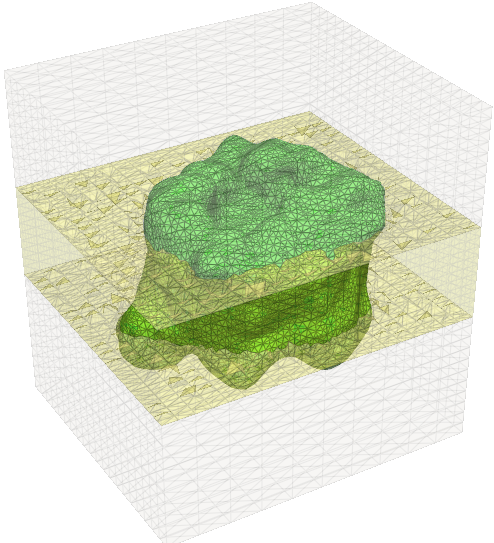
\includegraphics[width=0.89\linewidth]{figures/omega_plot.png}
                		\caption{A side view.}
                	\end{subfigure}
                    \begin{subfigure}[t]{0.3\linewidth}
                		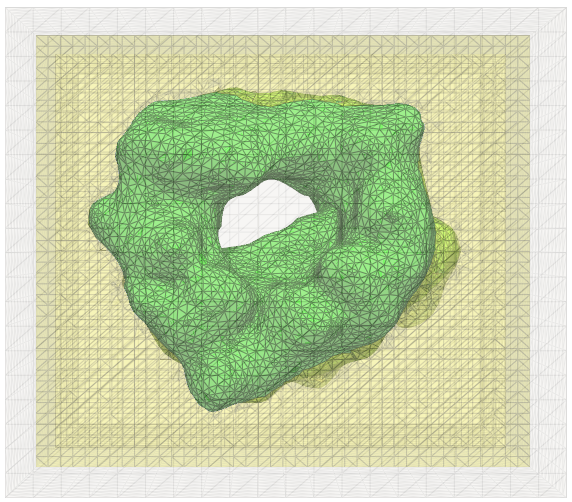
\includegraphics[width=0.89\linewidth]{figures/omega_plot_top.png}
                        %\vspace{5mm}
                		\caption{A top view.}
                	\end{subfigure}
                	\begin{subfigure}[t]{0.3\linewidth}
                		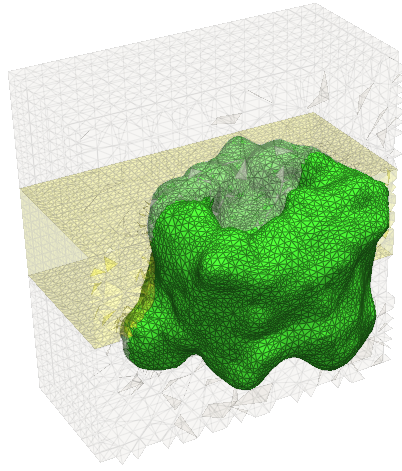
\includegraphics[width=0.84\linewidth]{figures/omega_plot_ds_clip.png}
                		\caption{A cropped view. }
                	\end{subfigure}
                	
                	\caption{Three views of the box domain mesh $\Omega_h$. Here, $D_{p,h}$, $D_{m,h}$, and $D_{s,h}$ are colored green, yellow, and gray, respectively, $D_{s,h}$ and $D_{m, h}$ are shown with low opacity to expose $D_{p,h}$ and $D_{m,h}$ partially; and $D_{s,h}$ is partially cropped to more clearly show the mesh structure of $D_{p,h}$.}
                \label{fig:3emn-mesh-views}
                    \end{figure}
                    
                \end{block}
                \vspace{2mm}
                \begin{block}{\centering \bf \large Nonlocal Relationship of Displacement and Electric Fields}

                The local Poisson ion channel models are based on linear dielectric relationships $\dd(\rr) = \ez \ep \ee(\rr)$ in $D_p,$ $\dd(\rr) = \ez \emem \ee(\rr)$ in $D_m,$ and $\dd(\rr) =\ez \es \ee(\rr)$ in $D_s.$ Here, $\dd$ is the displacement field, $\ee$ is the electric field, and $\ez, \ep, \emem, \es$ are permittivity constants. With $\Phi$ denoting the electrostatic potential function of $\ee$, we obtain a nonlocal dielectric relationship within $D_s$ as follows:
                \begin{equation*}
                    \dd(\rr) = \ez \int_{\mathbb{R}^3} \epsilon(\rr- \rp) \nabla \Phi(\rp)\mathrm{d}\rr, \qquad\text{for $\rr$ in $D_s$}  
                \end{equation*}
                 where $\epsilon$ is a nonlocal permittivity function given by 
                 \begin{equation*}
                      \epsilon(\rr) = \ei \delta + (\es - \ei)Q_\lambda(\rr).
                 \end{equation*}
                Here $\delta$ denotes the Dirac-delta distribution at the origin, $\ei$ and $\lambda$ are nonlocal parameters, and $Q_{\lambda}(\rr)=\frac{e^{-|\rr|/\lambda}}{4\pi \lambda^2 |\rr|}$, which is a Yukawa-type kernel satisfying
                \[ -\lambda^2\Delta Q_{\lambda}(\rr) + Q_{\lambda}(\rr) =\delta, \quad  \rr \in \mathbb{R}^{3}.\]
                \end{block}

            \end{column}
            \begin{column}{.32\linewidth}
                \begin{block}{\centering \bf \large Nonlocal Poisson Boltzmann Ion Channel Model}
                
                We scale $\Phi$ as a dimensionless potential $u$ to obtain the NPBIC model as follows:
                    \begin{equation*}
                    \label{NMPBic_u}
                     % \left\{
                     \begin{array}{cl}
                         -\epsilon_p\Delta u(\rr) =\alpha \sum\limits_{j=1}^{n_{p}}z_{j}  \delta_{\rr_{j}}(\rr), & \rr \in D_p,\\
                    -\epsilon_{\infty}\Delta u(\rr) + \frac{\epsilon_s-\epsilon_\infty}{\lambda^2}[u(\rr)-(u\ast Q_{\lambda})(\rr)]
                    = \beta \sum\limits_{i=1}^{n}Z_{i} c_{i}^{b} e^{-Z_{i} u(\rr)}, & \rr \in D_s,\\
                    -\epsilon_m \Delta u(\rr) = 0, & \rr \in D_m, \\
                    u(\s^{-}) = u(\s^{+}), \quad
                    \epsilon_p\frac{\partial u(\s^{-})}{\partial \nn_p(\s)} = \epsilon_\infty\frac{\partial u(\s^{+})}{\partial \nn_p(\s)}+(\epsilon_s-\epsilon_\infty)\frac{\partial (u\ast Q_{\lambda})(\s)}{\partial \nn_p(\s)}, & \s\in\Gamma_p,\\
                    u(\s^{-}) = u(\s^{+}), \quad \epsilon_m\frac{\partial u(\s^{-})}{\partial \nn_m(\s)} = \epsilon_\infty\frac{\partial u(\s^{+})}{\partial \nn_m(\s)}+(\epsilon_s-\epsilon_\infty)\frac{\partial (u\ast Q_{\lambda})(\s)}{\partial \nn_m(\s)}, & \s\in\Gamma_m,\\
                    u(\s^{-}) = u(\s^{+}), \quad  \epsilon_p\frac{\partial u(\s^{-})}{\partial \nn_p(\s)} = \epsilon_m\frac{\partial u(\s^{+})}{\partial \nn_p(\s)}, \quad &\s \in \Gamma_{pm}, \\
                       u(\s) = g(\s), & \s \in \Gamma_D, \\
                       \frac{\partial u (\s)}{\partial \nn_b(\s)} = 0, & \s \in \Gamma_N,
                    \end{array}
                    % \right.
                    \end{equation*}  
                    where $\alpha$ and $\beta$ are constants, $n_p$ is the number of atoms in a VDAC, $z_j$ is the charge number of atom $j$ at $\rr_j$, $n$ is the number of species of the ionic solution, $Z_i$ is the charge number of species $i$, and $(\Phi * Q_\lambda)(\rr) = \int_{\mathbb{R}^3}\Phi(\rp)Q_\lambda(\rr-\rp) \mathrm{d}\rp$. 
                    
                    %the NPBIC model to be reformulated as a local system of partial differential equations, without any convolution terms.  
                \end{block}
                \vspace{2mm}
                \begin{block}{\centering \bf \large Finite Element Solver and Program Package}
                    We have developed an efficient NPBIC finite element solver and implemented it as a Python package, enhanced by Fortran extension modules, based on the finite element library of the FEniCS project (Version 2019.1.0), our SMPBic program package, and our nonlocal modified PBE program package. The NPBIC package adapts ICMPv3 [1] to produce meshes $\Omega_h, D_{p, h}, D_{m, h}$ and $D_{s, h}$. 

                    \vspace{0.3em}
                    To avoid singularity difficulties caused by atomic charges, the NPBIC package calculate $u$ by the solution decomposition formula 
                    \[ u = G  + \Psi + \Phit,\]
                    where $G$ collects all the singularity points of $u$ as a known function, $\Psi$ is the solution to a linear nonlocal interface boundary value problem and $\Phit$ is the solution to a nonlinear nonlocal interface boundary value problem. The function $\Phit$ is found by a modified Newton iterative method, using an initial guess $\Phit^{(0)}$ generated from a local PB ion channel solution. 
                    % % \vspace{0.5em}
                \end{block}
                \vspace{2mm}
                \begin{block}{\centering \bf \large Numerical Test Results}
                
                 We conducted numerical experiments on two VDACs with PDB ID 3EMN and 2JK4. 3EMN is a mouse VDAC crystal structure, captured at 2.3 {\AA} resolution, consisting of 2,250 atoms and 283 residues. 2JK4 is a human VDAC crystal structure, captured at 4.10 {\AA} resolution, consisting of 2,207 atoms and 288 residues. For 3EMN, we set $\Omega = [-36, 43] \times [-36, 33] \times [-44, 40]$, and the mesh $\Omega_h$ contains $38,694$ vertices. For 2JK4, the mesh $\Omega_h$ contains $38,583$ vertices with $\Omega = [-39, 42] \times [-36, 37] \times [-50, 46]$. All tests were conducted in an ionic solution of 0.2 molar NaCl on one core of Mac mini with M4 chip. Test results are reported in Table~1 and Figures 1 to 4.

                  \vspace{2mm} 
                 
                    \begin{table}[]
                        \centering
                        \begin{tabular}{|c|c|c|c|c|c|}
                    \hline
                     PDBID & Find $G$, $\hat{G}, \nabla G, \nabla \hat{G}$ & Find $\Psi$ & Find $\Phit^{(0)}$ & Find $\Phit$ & Total \\
                    \hline
                    3EMN & 1.33 & 0.34 & 21.45 & 20.86 & 52.19 \\ \hline
                    2JK4 & 1.34 & 0.35 & 14.21 & 13.60 & 44.07 \\
                    \hline
                    \end{tabular}
                    \vspace{1mm}
                        \caption{Performance of our NPBIC package for 3EMN and 2JK4 in terms of computer CPU time (in seconds). Here, ``Total" denotes the total CPU time.}
                        \label{table:time-table}
                    \end{table}
                    
                \end{block}
                
            \end{column}
            \begin{column}{0.32\linewidth}
                
                \begin{blockwithouttitle}{} %{\center \bf \large \color{blue} Results}
                
                         \begin{figure}
                    	\centering
                    	\begin{subfigure}{0.4\linewidth}
                    		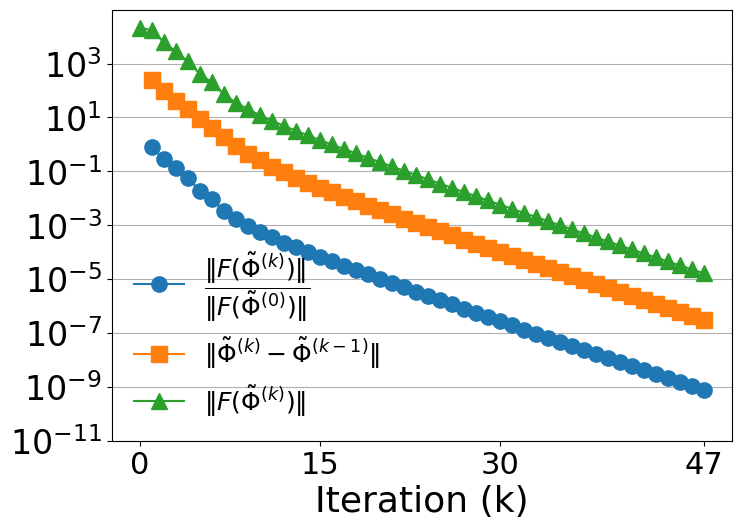
\includegraphics[width=\linewidth]{figures/3emn_convergence.png}
                    		\caption{Convergence for VDAC 3EMN.}
                    	\end{subfigure}
                        \hspace{8mm}
                    	\begin{subfigure}{0.4\linewidth}
                    		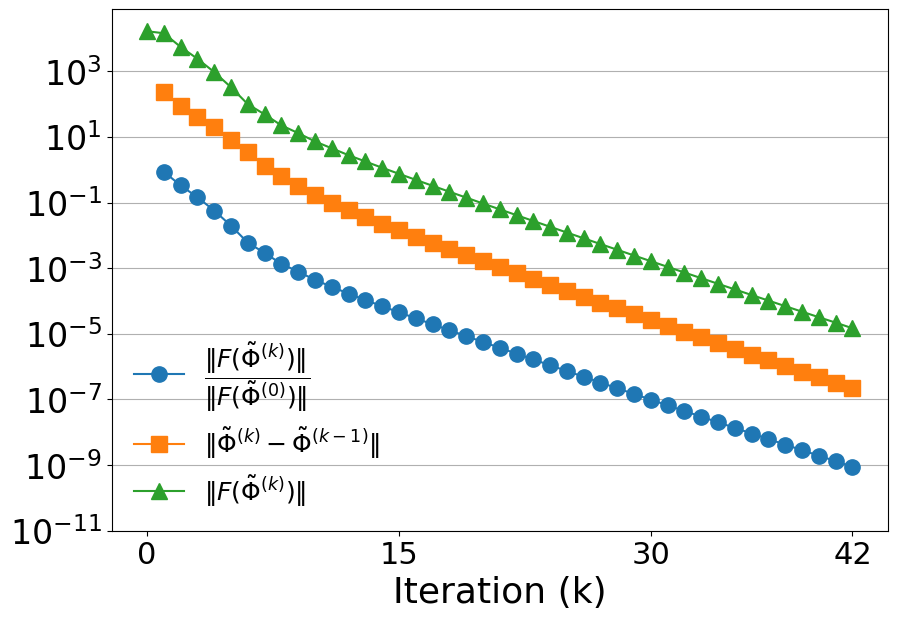
\includegraphics[width=\linewidth]{figures/2jk4_convergence.png}
                    		\caption{Convergence for VDAC 2JK4.}
                    	\end{subfigure}
                    	\caption{Convergence processes of our modified Newton iterative method for computing $\Phit$ in three errors: the relative residual error $\|F(\Phit^{(k)})\| / \|F(\Phit^{(0)})\|$, the error $\|\Phit^{(k)} - \Phit^{(k-1)}\|$, and the absolute residual error $\|F(\Phit^{(k)})\|$. Here $\Phit^{(k)}$ denotes the $k$th iterative approximation to $\Phit$.}
                    \label{fig:newton-convergence}
                    \end{figure}
                    
                    % Figure~\ref{fig:heatmaps} shows the electrostatic potential function $u$ as well as the concentration of Na$^+$ and Cl$^-$ for the VDAC 3EMN. 
                    
                    \begin{figure}
                         \begin{subfigure}[t]{0.3\linewidth}
                            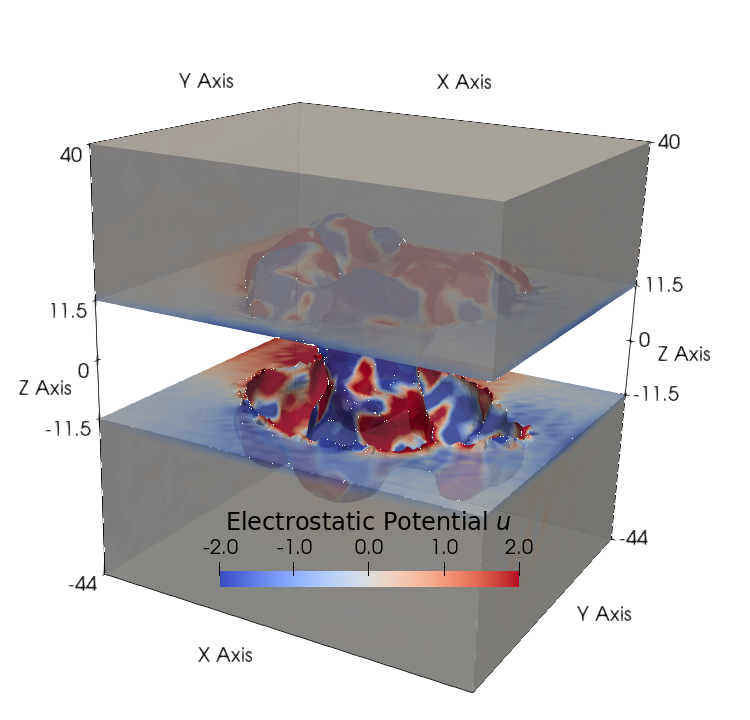
\includegraphics[width =\linewidth]{figures/u_cmap.png}
                            % \caption{Surface of $u.$}
                        \end{subfigure}
                        \begin{subfigure}[t]{0.3\linewidth}
                            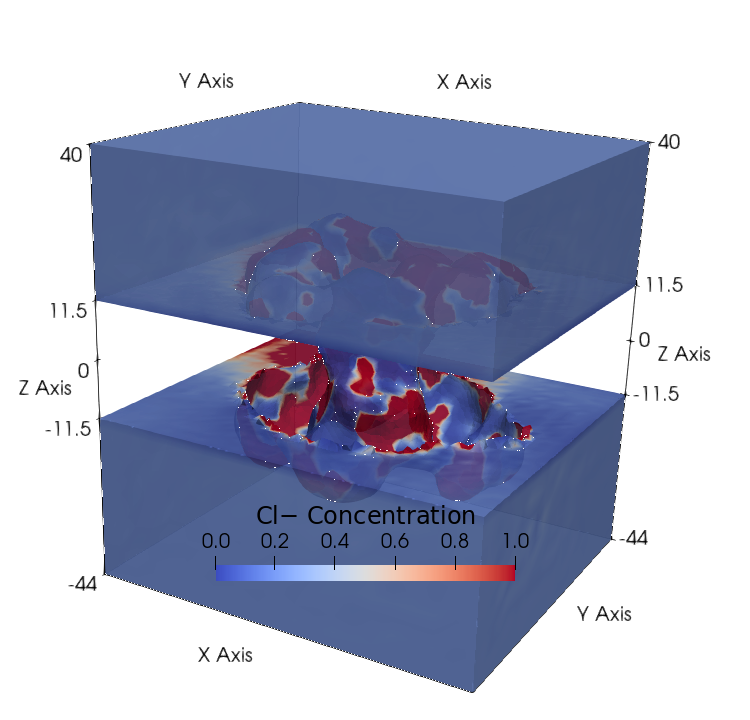
\includegraphics[width =\linewidth]{figures/cl_cmap.png}
                            % \caption{Surface of $u.$}
                        \end{subfigure}
                        \begin{subfigure}[t]{0.3\linewidth}
                            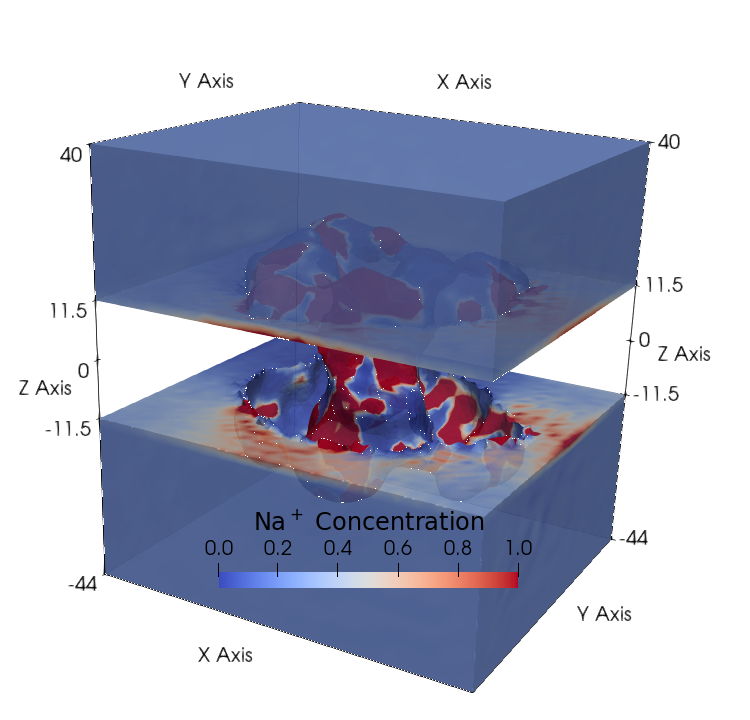
\includegraphics[width =\linewidth]{figures/na_cmap.png}
                            % \caption{Surface of $u.$}
                        \end{subfigure}
                        \vspace{2mm}
                        \caption{Color-mappings of the NPBIC finite element solution $u$ and the concentrations of Na$^+$ and Cl$^-$ in molar, determined by $u$, for 3EMN, confirming the anion selectivity of VDAC.}\label{fig:heatmaps}
                    \end{figure}
                    
                    \vspace{1em}
                    \begin{figure}
                    
                        \centering
                        \begin{subfigure}[t]{0.3\linewidth}
                            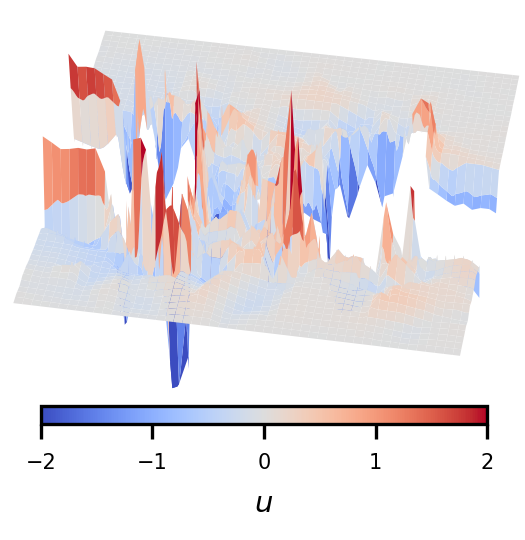
\includegraphics[width =\linewidth]{figures/nonlocal_potDs.png}
                            \caption{Surface of $u.$}
                        \end{subfigure}
                        \begin{subfigure}[t]{0.3\linewidth}
                            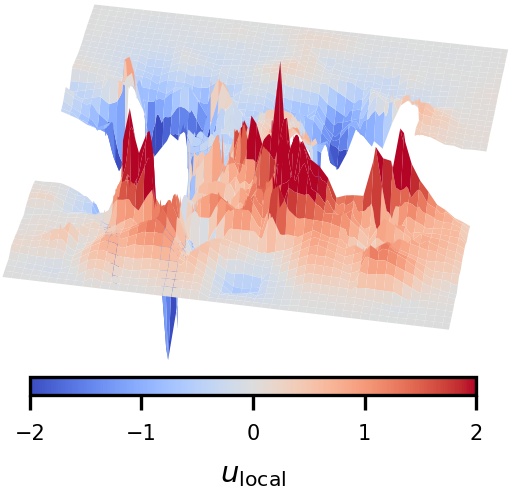
\includegraphics[width =\linewidth]{figures/local_potDs.png}
                            \caption{Surface of $u_{loc}.$}
                        \end{subfigure}
                        \begin{subfigure}[t]{0.3\linewidth}
                            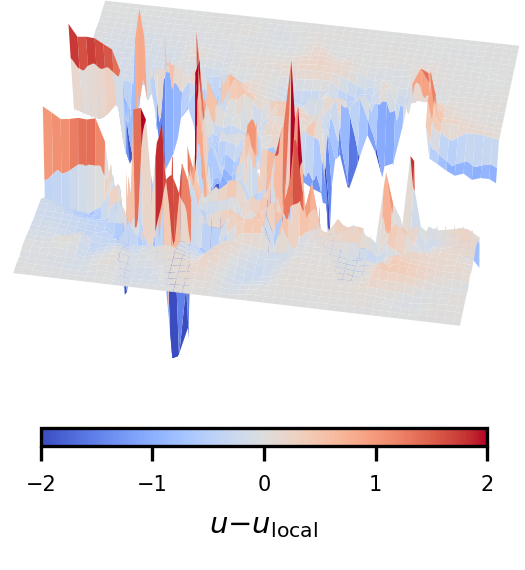
\includegraphics[width =\linewidth]{figures/comp_potDs.png}
                            \caption{Surface of $u - u_{loc}.$ }
                        \end{subfigure}
                        \caption{A comparison of the NBPic solution $u(0, y, z)$ with the local PBic solution $u_{loc}(0, y, z)$ for $(y, z)$ in a slice ($x=0$) of $D_s$. Here $u$, $u_{loc}$ and $u-u_{local}$ are plotted as surfaces, showing that the NPBIC model produces a significantly different electrostatic potential function. }\label{fig:surfaces}
                    \end{figure}

                    We plan to use our NPBIC package to compute electrostatic solvation free energies, making  it a valuable tool in various biological applications.
                   
                \end{blockwithouttitle}
                \vspace{2mm}
                \begin{block}{\centering \bf \large Acknowledgments}
                    This work was partially supported by the US National Science Foundation through the award number DMS-2153376.
                    \vspace{0.3em}
                    
                    The author L. Jemison thanks the National Institute for Theory and Mathematics in Biology for the generous travel support. 

                    \vspace{0.3em}
                    For questions email \url{ljemison@uwm.edu} and \url{dxie@uwm.edu}. 

                    \vspace{0.7em}
                    [1] L. Jemison, M. Stahl, R. K. Dash, and D. Xie, Vol. 41 (1), e70003, Journal of Computational Chemistry, 2025.

                    \vspace{1.55em}
                \end{block}
            \end{column}
         \end{columns}
   \end{frame}
 
  
\end{document}